%==============================
\section{MILP}

Mathematical Models: Given a poset $P=(\Omega,\preceq_{\varphi},\neq_{\varphi})$, where $\Omega$ is a sequence of 
subtasks, and~$\preceq_{\varphi}$, $\neq_{\varphi}$ are the partial relations to describe the temporal order 
between the subtasks.
 $\omega_1\preceq_{\varphi}\omega_2$ means subtask $\omega_2$ should begin after the start of 
 $\omega_1$ and $\omega_1\neq_{\varphi}\omega_2$ means the execution time of $\omega_1,\omega_2$ should not have
 intersection. 
An agent swarm is required to execute these subtasks under the constrains of 
$\preceq_{\varphi},\neq_{\varphi}$ in a $300\times500$ work space \ref{workspace}. 
Additionally, the agents are heteroid as there are three different agent type $V_f,V_l,V_s$
with different velocity and different functions. 
For any subtask $\omega_j\in\Omega$, it needs a particular combination of 
different type of collaborators as showed in table~\ref{fig:symbols}.
The optimal function is to minimum the max execution time of subtasks $\Omega$.
To go further, we give the table of definition for the symbols in this mathematical models.
\begin{table}[t]
	\centering
	\caption{Description of related regions and agent actions.}
	\label{fig:symbols}
	\begin{tabular}{|c|m{0.5\columnwidth}|c|}\hline
		\textbf{Proposition} & \textbf{Description}\centering & \textbf{Duration} [s]\\ \hline
		$\texttt{p}_1,\cdots,\texttt{p}_{34}$ & $34$ PV panels. & $\backslash$ \\ \hline
		$\texttt{b}$ & Base stations for all agents to park and charge. & $\backslash$ \\ \hline
		$\texttt{t}_1,\cdots,\texttt{t}_7$ & $7$ transformers. & $\backslash$ \\ \hline
		$\texttt{temp}_{\texttt{p}_i,\texttt{t}_i}$ &
		Measure temperature of panel~$\texttt{p}_i$ and transformer $\texttt{t}_i$.
		Requires one~$V_f$. & 10 \\ \hline
		$\texttt{sweep}_{\texttt{p}_i}$& Sweep debris around any panel~$\texttt{p}_i$.
		Requires one $V_s$. & 190\\ \hline
		$\texttt{mow}_{\texttt{p}_i,\texttt{t}_i}$ &
		Mow the grass under panel~$\texttt{p}_i$ or transformer~$\texttt{t}_i$.
		Requires one $V_s$. & 190\\ \hline
		$\texttt{fix}_{\texttt{t}_i}$ &
		Fix malfunctional transformer~$\texttt{t}_i$.
		Requires one $V_l$ and one $V_s$ & 72\\ \hline
		$\texttt{repair}_{\texttt{p}_i}$ &
		Repair broken panel~$\texttt{p}_i$.
		Requires one $V_s$ to repair and two $V_f$ to guide. & 576\\ \hline
		$\texttt{wash}_{\texttt{p}_i}$ &
		Wash the dirt off panel~$\texttt{p}_i$.
		Requires one $V_l$ to wash and one $V_f$ to monitor the progress. & 565\\ \hline
		$\texttt{scan}_{\texttt{p}_i,\texttt{t}_i}$ &
		Build 3D models of panel~$\texttt{p}_i$ or transformer~$\texttt{t}_i$
		for inspection. Requires three $V_f$. & 95\\ \hline
	\end{tabular}
\end{table}
\begin{figure}
	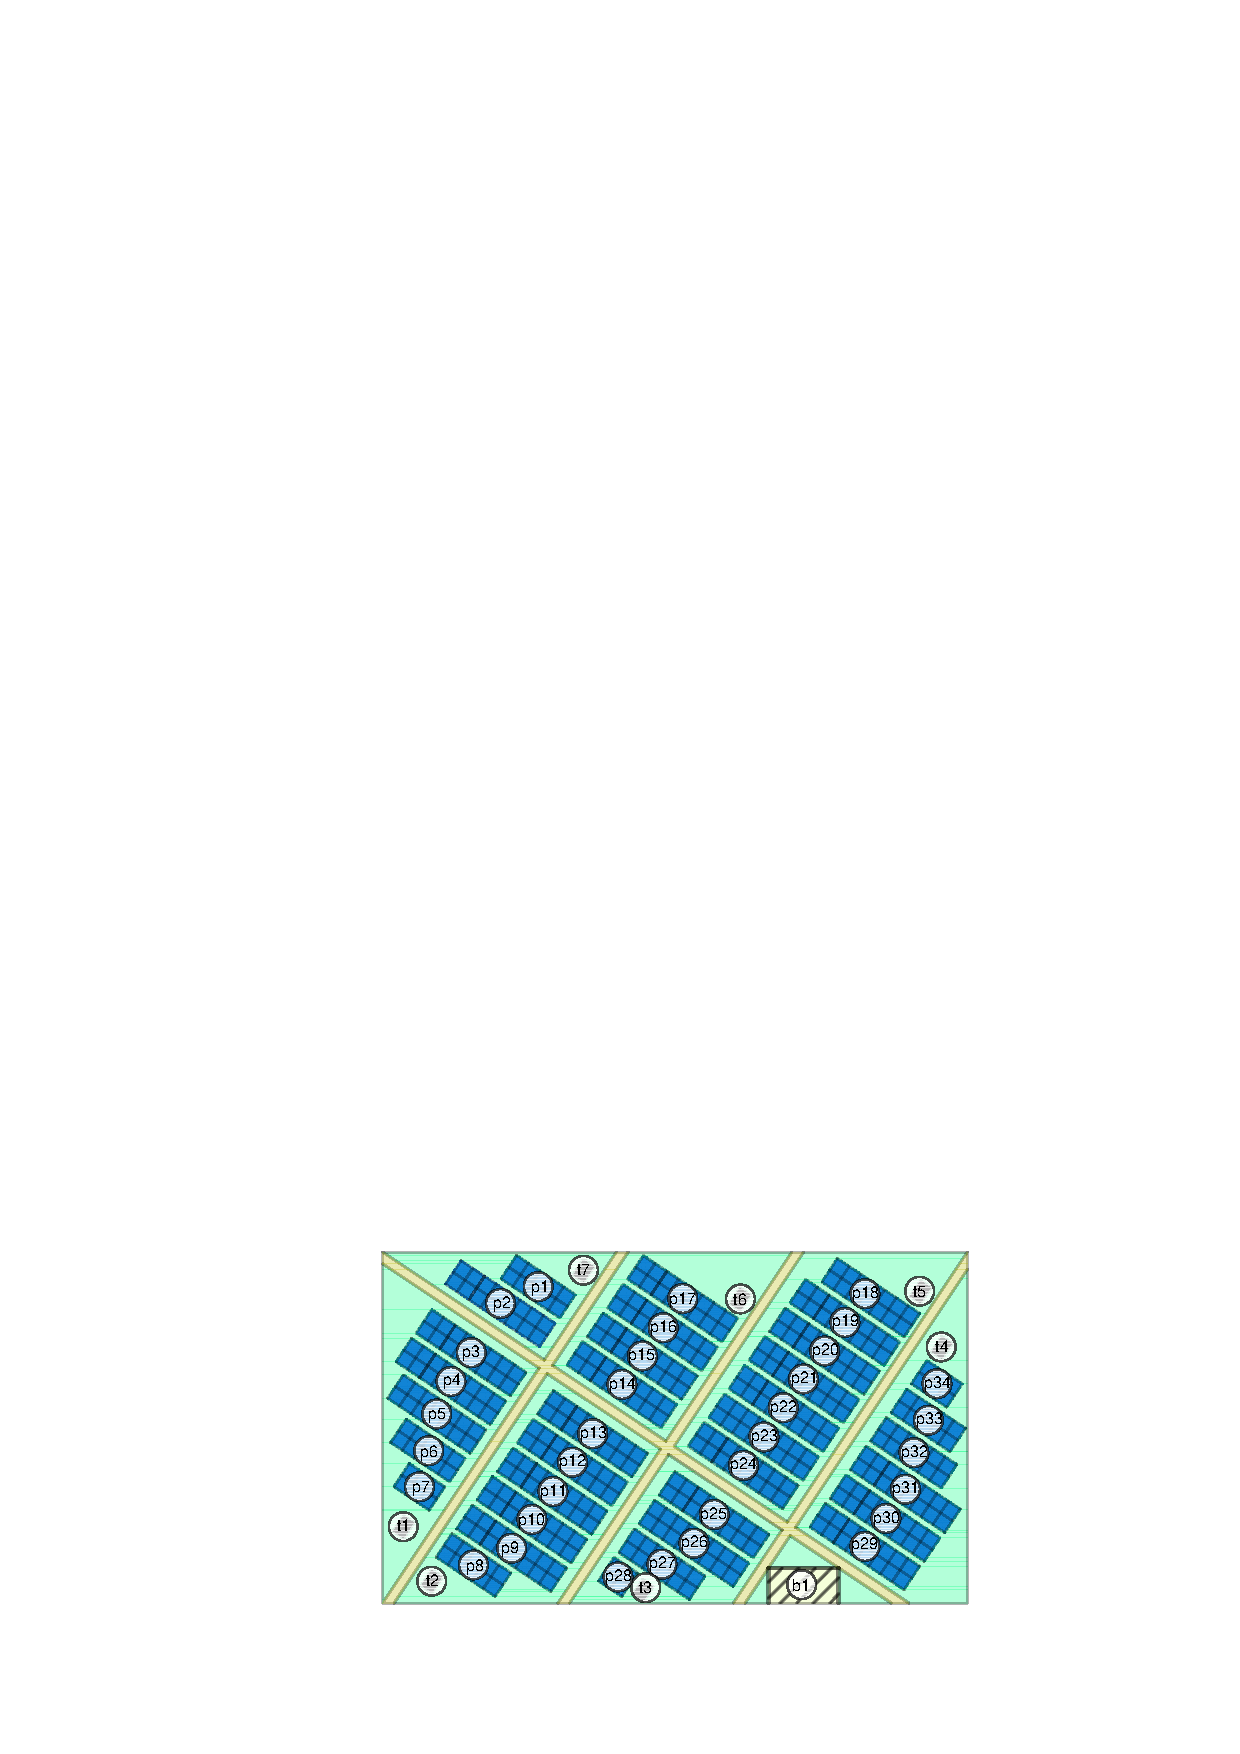
\includegraphics[width=0.36\textheight]{figure/background.pdf}
	\caption{Work space}
	\label{workspace}
\end{figure}

\begin{table}[h]
	\begin{tabular}{|l|p{0.5\columnwidth}|p{0.2\columnwidth}|}\hline
		Variable &\multicolumn{2}{c|}{ Variable definition }\\\hline
		Name & definition & range \\
		$P$ & partial order set& \\
		$m$  & number of agents & $\mathcal{N}$\\
		$n$ & number of tasks & $\mathcal{N}$ \\
			$i$ & agent $i$ & $i\leq n$\\
		$j$ & task $j$ & $j\leq m$	\\
		$k$ & order of tasks & $j\leq m$\\
		$o$ & number of serves type agent can provide & $ \mathcal{N}$\\
		$l$ & order of tasks & $j\leq o$\\
		$\Omega$ & set of subtasks &\\
		$q_{j_1,j_2}$ &task $j_1$ execute in front of $j_2$ or not& $\{0,1\}$\\
		$T_b$ & a pretty large number as time budget & $T_b>0$ \\ 
		$r_{i,j,k,l}$ & agent $i$ execute task $j$ providing serve $l$ in the order $k$ & $\{0,1\}$\\
		$t_j$ & begin time of task $j$ & $t_j>0$ \\
		$p_j$ & continue time of task $j$ & $p_j >0$\\
		$a_{j,l}$ & number of servey $l$ task $j$ needed. & $\mathcal{N}$\\
		$b_{i,l}$ & type of servey $l$ that agent $i$ can provide & $\{0,1\}$ \\
		$v_i$ & velocity of agent $i$ &   $v_i>0$\\
		$dis_{j_1,j_2}$ & distance from task $j_1$ to task $j_2$ &  $dis_{j_1,j_2}>0$\\
		$dis_{i,j}$ & distance from initial $i$ to task $j$ & $dis_{i,j}>0$\\\hline
	\end{tabular}
	\centering
	\caption{variable definition}
	\label{tab:Margin_settings}
\end{table}
\begin{equation}
\min_{r_{i,j,k,l}, t_j,q_{j_1,j_2}}  \max(t_j+p_j)
\label{0}
\end{equation}
s.t.\\
$\preceq_{\varphi}$ constraint of tasks:
\begin{equation}
t_{j_1}+p_{j_1}\leq t_{j_2} \quad  \forall (j_1,j_2)\in \preceq_{\varphi}\\
\label{1}
\end{equation}
$\neq_{\varphi}$ constraint of tasks:
\begin{equation}
t_{j_1}+p_{j_1}+q_{j_1,j_2}T_b\leq t_{j_2}\quad  \forall (j_1,j_2)\in \neq_{\varphi}\\
\label{1.5}
\end{equation}
\begin{equation}
t_{j_2}+p_{j_2}+(q_{j_1,j_2}-1)T_b\leq t_{j_1} \quad  \forall (j_1,j_2)\in \neq_{\varphi}\\
\label{1.8}
\end{equation}
provide enough serves for the task $j$
\begin{equation}
\sum_{i=1}^{m}\sum_{k=1}^{n}r_{i,j,k,l}b_{i,l}= a_{j,l}   \quad \forall j,l
\label{2}
\end{equation}
one agent can only provide the serve it has:
\begin{equation}
r_{i,j,k,l}\leq b_{i,l}   \quad \forall i,j,k,l
\label{3}
\end{equation}
One agent can execute one task no more than once:
\begin{equation}
\sum_{k=1}^{n}\sum_{l=1}^{o}r_{i,j,k,l} \leq 1   \forall i,j
\label{4}
\end{equation}
One agent at any time can execute no more than one task:
\begin{equation}
\sum_{j=1}^{m}\sum_{l=1}^{o}r_{i,j,k,l} \leq 1    \forall i,k
\label{5}
\end{equation}
One agent can execute $k+1th$ task only if it execute $kth$ task.
\begin{equation}
\sum_{j=1}^{m}\sum_{l=1}^{o}r_{i,j,k,l} - \sum_{j=1}^{m}\sum_{l=1}^{o}r_{i,j,k+1,l}\leq  0    \qquad\forall i,k<m-1
\label{6}
\end{equation}
Even agent need to obey the motion constrain.
\begin{equation}
\begin{aligned}
&t_{i_2}-t_{i_1} -M\sum_{l=1}^o r_{i,j_1,k,l}-M\sum_{l=1}^o r_{i,j_2,k+1,l}  \geq\\
& dis_{j_1,j_2}/v+p_{i_1}-2M \quad   \forall i,j
\end{aligned}
\label{7}
\end{equation}
\begin{equation}
t_{i} -M\sum_{l=1}^o r_{i,j,1,l} \geq dis_{i,j}/v-M \qquad  \forall i,j
\label{8}
\end{equation}

With the constraints mentioned above, we defined this Mixed interger linear programming(MILP) question. 
Unfortunately, duo to the number of bool variables
is $MN^2O$, the complexity of this question is exploding as agent number $M$ or task number $N$ increase.
 


\section{Lower Bound method}
\label{lower bound method}
Here we put out another Lower Bound method which is more complex than the one in article but is more accurate. This
method preforms better in the small agent swarm and subtasks that $MN\leq 50$ because it can return a more accurate
lower bound but it's performance descent tepidly in larger scale system as $MN\geq 100$. 
Comparing to the original question~\ref{0}~\ref{8}, we use a simplified mathematical model.  
Instead of calculating the distance cost caused by different tasks order, we use the time lower
bound $t_{low}$ instead. $t_{low}$ is the minimum time for any agent to go to the goal place.
   The lower bound is consisted of two parts, the first is to calculate the exact solution of current node. The
second part is to estimate the makespan based on current boundary condition. The first part is an algorithm of P-hard.
We only need to consider the partial order in the assigned tasks and motion constrains. For the partial order constrain:

$$\min_{t_{j_a}} \quad \max(t_{j_a}+p_{j_a})$$
s.t.\\

\begin{equation}
 t_{j_a1} + p_{j_a1}< t_{j_a2}   \quad \forall j_{a1}, j_{a2} \in P , j_{a1} \in N_a, j_{a2} \in N_a
\label{9}
\end{equation}

When task $j$ is the first task of agent $i$, the motion constrain is :
\begin{equation}
dis_{i,j_a}/v_i+ p_{j_a}< t_{j_a}
\label{10}
\end{equation}

When task $j_{a2}$ is the next task of task $t_{a1}$ in agent $i$, the motion constrain is:

\begin{equation}
dis_{j_{a1},j_{a2}}/v_i+ p_{j_{a1}}+t_{j_{a1}}- t_{j_{a2}}<0
\label{11}
\end{equation}

Then we can generate the $t_{i0}$ of each agent, which means the time agent finished assigned tasks
 and can begin to execute the left unassigned tasks.$t_{j_i}$ is the assigned task to the agent $i$.
We defined that the task set assigned to agent $i$ is $T_i$.
\begin{equation}
t_{i0} = \max{\{t_{j_a}\}}    \quad {j_a}\in T_i
\label{12}
\end{equation}

To the unassigned task, we propose an algorithm with much simplified to get the final lower bound.
Instead of consider the order relationship of task, we use the lower bound of motion cost to unify
the executing time for one task in any order. That is rebuilding the task executing time $p_j$ with
a minimum possible motion cost as $p'_j$.

\begin{equation}
p'_j = \min{\{\frac{dis_{i,j}}{v_i}, \frac{dis_{j_1,j_2}}{\max{v_i}}\}}+p_j    \quad \forall j\in N_u, \forall i \in \mathcal{M}
\label{13}
\end{equation}

Thus, the optimal function and constrains are in the following:
\begin{equation}
\min_{r_{i,j},t_i} \quad \max(t_i)
\label{14}
\end{equation}

s.t.\\

Enough executor constrain:
\begin{equation}
  \sum_{i=1}^{m}r_{i,j} = a_{j}  \forall j \in N_u
  \label{15}
\end{equation}

Relaxed motion and task executing time constrain:

\begin{equation}
\sum_{j=1}^{n}r_{i,j}p'_j +t_i > t_{i0} \forall i \in \mathcal{M}
\label{16}
\end{equation}

The complexity of first part is $O(N_a)$, and the complexity of the second part is $O(N_u*M)$.
Comparing to \ref{0}, we ignore the order relations between tasks so that the execution of
each task is compact and the poset constrains is neglected. Also, we relaxed the sub-task type
constrains as \ref{2},\ref{3},\ref{4} and only require enough agent execute a cooperative task
as \ref{15}. Also, we do not require a cooperation task to execute at same time in different
agents thus the optimal value is certainly smaller than the MILP. 

\begin{table}[h]
	\begin{tabular}{|l|p{0.5\columnwidth}|p{0.2\columnwidth}|}\hline
		Name & Variable definition & range \\\hline
		$P$ & partial order set& \\
		$M$  & number of agents & $\mathcal{N}$\\
		$\mathcal{M}$  & agent set & \\
		$N_a$ & set of assigned tasks &  \\
		$N_u$ & set of unassigned tasks &  \\
		$T_i$ & assigned tasks for agent $i$ &  \\

		$n_u$ & number of unassigned tasks & $\mathcal{N}$ \\
		$t_{j_a}$ & finished time of assigned tasks & $t_{j_a}>0$\\
		$\Omega$ & anchor function &\\
		$r_{i,j}$ & agent $i$ execute task $j$ & $\{0,1\}$\\
		$t_{i0}$ & begin time of agent $i$ & $t_i>0$ \\
		$t_i$ & end time of agent $i$ & $t_i>0$ \\
		$p_j$ & continue time of task $j$ & $p_j >0$\\
		$p'_j$ & estimate continue time of task $j$ & $p_j >0$\\
		$a_{j}$ & number agent task $j$ needed. & $\mathcal{N}$\\
		$v_i$ & velocity of agent $i$ &   $v_i>0$\\
		$dis_{j_1,j_2}$ & distance from task $j_1$ to task $j_2$ &  $dis_{j_1,j_2}>0$\\
		$dis_{i,j}$ & distance from initial $i$ to task $j$ & $dis_{i,j}>0$\\\hline
	\end{tabular}
	\centering
	\caption{variable definition}
	\label{}
\end{table}




